\documentclass[12pt]{article}
\usepackage[utf8]{inputenc}
\usepackage{amsmath}
\usepackage{amssymb}
\usepackage{graphicx}

\graphicspath{ {./plots/} }

\newcommand{\rectres}[1]{
\begin{center}
\begin{tabular}{ |c| }
\hline\\
#1\\
\\
\hline
\end{tabular}
\end{center}
}

\newcommand{\qed}{\hfill$\blacksquare$}

\title{Introduction to Numerical Optimization\\Assignment 2}
%\author{Yair Nahum 034462796\\and\\blabla 11111111 }

\begin{document}

\maketitle

%\tableofcontents{}

\section{Convex Sets and Functions}

\subsection{Question 1}
Need to prove that if we have 2 convex functions $f_1$ and $f_2$ over convex set $C$, then $$g(x)=\max\limits_{i=1,2} f_i(x)$$ is also a convex function over convex set $C$
\subsubsection*{Proof}
Let's pick some points $s,t \in C$\\
We need to show that $$g(\alpha s + (1-\alpha)t) \leq \alpha g(s) + (1-\alpha)g(t) \hspace{20} \forall \alpha \in [0,1]$$
$f_1$ is convex $\Rightarrow$
$$f_1(\alpha s + (1-\alpha)t) \leq \alpha f_1(s) + (1-\alpha)f_1(t)$$
$f_2$ is convex $\Rightarrow$
$$f_2(\alpha s + (1-\alpha)t) \leq \alpha f_2(s) + (1-\alpha)f_2(t)$$
Since each function is convex in that intermediate point $(\alpha s + (1-\alpha)t)\in C$, we can only increment each max argument and deduce:
$$g(\alpha s + (1-\alpha)t) = \max\limits_{i=1,2} f_i(\alpha s + (1-\alpha)t) \leq \max\limits_{i=1,2} \{\alpha f_i(s) + (1-\alpha)f_i(t)\} $$
Now, since $a \leq max(a,c)$ and $b \leq max(b,d)$ we have the following identity:\\
$$a+b \leq max(a,c)+max(b,d)$$
In the same way we get:\\
$$c+d \leq max(a,c)+max(b,d)$$
And thus:
$$max(a+b,c+d) \leq max(a,c)+max(b,d)$$
Therefore:
$$\max\limits_{i=1,2} \{\alpha f_i(s) + (1-\alpha)f_i(t)\} \leq \max\limits_{i=1,2} \{\alpha f_i(s)\} + \max\limits_{i=1,2} \{ (1-\alpha)f_i(t)\}$$
We continue by getting scalars out:
$$\max\limits_{i=1,2} \{ \alpha f_i(s) \} + \max\limits_{i=1,2}\{(1-\alpha)f_i(t)\} = \alpha \max\limits_{i=1,2} f_i(s) + (1-\alpha)\max\limits_{i=1,2} f_i(t) = \alpha g(s) + (1-\alpha)g(t)$$
\qed\\
Another way to prove it is by contradiction.
\subsubsection*{Proof}
Assume $g(x)$ is not convex. Meaning, $$\exists s,t \in C \text{ and } \exists \alpha \in [0,1] \text{  s.t.}$$ 
$$g(\alpha s + (1-\alpha)t) > \alpha g(s) + (1-\alpha)g(t)$$
On the other hand, $\forall i \in \{1,2\}$ 
$$\alpha g(s) + (1-\alpha)g(t) = \alpha \max\limits_{j=1,2} f_j(s) + (1-\alpha)\max\limits_{j=1,2} f_j(t) \geq \alpha  f_i(s) + (1-\alpha)f_i(t) \geq f_i(\alpha s + (1-\alpha)t)$$
When the last inequality is due to convexity of $f_i$
So using our assumption and the above, we get that $\forall i \in \{1,2\}$:
$$g(\alpha s + (1-\alpha)t) > f_i(\alpha s + (1-\alpha)t)$$
In contradiction to the definition of $g(x)$ that must be equal to one of the $f_i$ functions as:
$$g(x)=\max\limits_{i=1,2} f_i(x)$$
Therefore $g(x)$ must be convex.

\qed\\
\newpage
\subsection{Question 2}
Let $f(x)$ be a convex function defined over convex domain $C$\\
We need to show that the level set $L = \{x \in C, f(x) \leq \alpha \}$ is a convex set.
Meaning, we need to prove that for any $y,z \in L$:
$$\beta y + (1-\beta)z \in L \:\:\:, \forall \beta \in [0,1]$$
That is:\\
(1)$\:\:\:\beta y + (1-\beta)z \in C$\\
$\text{ and }$\\
(2)$\:\:\:f(\beta y + (1-\beta)z) \leq \alpha$
\subsubsection*{Proof}
(1) From definition of $L$ and $C$:
$$\:\:\: y,z \in L \Rightarrow y,z \in C \Rightarrow \beta y + (1-\beta)z \in C$$
(2) Due to $f$ convexity over $C$ (first inequality) and $y,z \in L$ (second inequality):
$$f(\beta y + (1-\beta)z) \leq \beta f(y) + (1-\beta)f(z) \leq  \beta \alpha  + (1-\beta)\alpha = \alpha$$
\qed\\

\newpage
\subsection{Question 3}
Let $f(x)$ be a smooth and twice differential convex function over a convex domain $C$.\\
We need to prove that $g(x) = f(Ax)$ is convex, where A is a matrix of appropriate size.
\subsubsection*{Proof}
As we learned in class, a function is convex if and only if its Hessian is PSD (we proved in class one direction but it's correct also on the other direction).\\
So, we will show that $\nabla^2 g(x)$ is PSD.\\
That is, we need to show that:
$$\forall z \in \mathbb{R}^n, \;\;\; z^T \nabla^2 g(x) z \geq 0$$
As we learned, if $g(x) = f(Ax)$, then 
$$\nabla^2 g(x) = A^T \nabla^2 f(x) A \Rightarrow$$
$$z^T \nabla^2 g(x) z = z^T A^T \nabla^2 f(x) A z$$
We can denote $y = Az$ and get:
$$z^T \nabla^2 g(x) z = y^T \nabla^2 f(x) y \geq 0$$
When the last inequality is due to convexity of $f(x)$\\
$\text{ }$\qed

\newpage
\subsection{Question 4}
Jensen's inequality states the following:\\
Let $f:C \rightarrow \mathbb{R}$ be a convex function over a convex set domain $C \in \mathbb{R}^n$.\\
Then, for any collection of points $x_1,x_2,..,x_k \in C$ and any collection of positive scalars $\alpha_1,\alpha_2,..,\alpha_k$ s.t. $\sum_{i=1}^k \alpha_i = 1$\\
We have:
$$f(\sum_{i=1}^k \alpha_i x_i) \leq \sum_{i=1}^k \alpha_i f(x_i)$$
\subsubsection*{Proof}
We prove it by induction.\\
Base:\\
for $k=2$ it is trivial as $f(x)$ is convex and therefore:
$$f(\alpha_1 x_1 + \alpha_2 x_2) = f(\alpha_1 x_1 + (1-\alpha_1) x_2) \leq \alpha_1 f(x_1) + (1-\alpha_1) f(x_2) = \alpha_1 f(x_1) + \alpha_2 f(x_2)$$
Assumption:\\
We assume correctness of Jensen's inequality for $k-1$. Meaning,
$$f(\sum_{i=1}^{k-1} \alpha_i x_i) \leq \sum_{i=1}^{k-1} \alpha_i f(x_i)$$
Step:\\
We denote $$y=\sum_{i=1}^{k-1} \frac{\alpha_i}{(1-\alpha_k)} x_i$$ Thus,
$$f(\sum_{i=1}^{k} \alpha_i x_i) = $$
$$f(\sum_{i=1}^{k-1} \alpha_i x_i + \alpha_k x_k) = $$
$$f(\sum_{i=1}^{k-1} \alpha_i x_i + \alpha_k x_k) =$$
$$ f((1-\alpha_k)\sum_{i=1}^{k-1} \frac{\alpha_i}{(1-\alpha_k)} x_i + \alpha_k x_k) =$$
$$f((1-\alpha_k)y + \alpha_k x_k)$$
Also, $y\in C$ since $x_i \in C$ and
$$\sum_{i=1}^{k-1} \frac{\alpha_i}{(1-\alpha_k)}=1$$
So, due to convexity of 2 points in $C$ we get:
$$f(\sum_{i=1}^{k} \alpha_i x_i) = $$
$$f((1-\alpha_k)y + \alpha_k x_k) \leq$$
$$(1-\alpha_k)f(y) + \alpha_k f(x_k) = $$
$$(1-\alpha_k) f(\sum_{i=1}^{k-1} \frac{\alpha_i}{(1-\alpha_k)} x_i) + \alpha_k f(x_k) \leq_{(***)}$$
$$(1-\alpha_k) \sum_{i=1}^{k-1} \frac{\alpha_i}{(1-\alpha_k)} f(x_i) + \alpha_k f(x_k) =$$
$$\sum_{i=1}^{k} \alpha_i f(x_i)$$
When we used the induction assumption at the last inequality marked with $(***)$
\qed
\newpage

\subsection{Question 5}
Using Jensen’s inequality, we need to prove the arithmetic/geometric mean inequality:
$$\frac{\sum_{i=1}^n x_i}{n} \geq \sqrt[n]{\prod_{i=0}^n x_i}$$
Where $\forall i : x_i >0$
\subsubsection*{Proof}
First, we will show that $f(z)=-\log{(z)}:\mathbb{R}^n \rightarrow \mathbb{R}$ is convex.\\
The gradient of $-log(z)$ can be calculated from the definition:\\
$$d(f(z)) = -d(\log{(z)}) = -(\frac{1}{z_1},\frac{1}{z_2},..,\frac{1}{z_n})dz\Rightarrow$$
$$\nabla (-log(z)) = -(\frac{1}{z_1},\frac{1}{z_2},..,\frac{1}{z_n})^T$$
The hessian of $-log(z)$ can be calculated from the definition as well and we get a diagonal matrix in which all the entries on the diagonal are positive (as it is assumed that $z_i > 0$):\\
$$
\nabla^2 (-log(z)) =
\begin{pmatrix}
    \frac{1}{z_1^2} & 0 & .. & 0 \\
    0 & \frac{1}{z_2^2} & .. & 0\\
    ...\\
    0 & 0 &  .. & \frac{1}{z_n^2}
\end{pmatrix}
\Rightarrow$$
for any $u \in \mathbb{R}^n, u \neq 0$:\\
$$u^T \nabla^2 (-log(z)) u = \sum_{i=1}^n \frac{1}{z_i^2} u_i^2 \geq 0 \Rightarrow$$
$\nabla^2 (-log(z))$ is PSD $\Rightarrow -log(z)$ is convex.\\ 
\\
Second, from Jensen's inequality on convex function, the following is true $(\alpha_i = \frac{1}{n})$:\\
$$-\log(\frac{1}{n} \sum_{i=1}^n x_i) \leq -\sum_{i=1}^n \frac{1}{n} \log(x_i) \Rightarrow$$
$$-\log(\frac{1}{n} \sum_{i=1}^n x_i) \leq -\frac{1}{n} \sum_{i=1}^n \log(x_i) \Rightarrow$$
$$-\log(\frac{1}{n} \sum_{i=1}^n x_i) \leq -\frac{1}{n} \log(\prod_{i=1}^n x_i) \Rightarrow$$
$$-\log(\frac{1}{n} \sum_{i=1}^n x_i) \leq -\log(\{\prod_{i=1}^n x_i\}^\frac{1}{n}) \Rightarrow$$
$$-\log(\frac{1}{n} \sum_{i=1}^n x_i) \leq -\log(\sqrt[n]{\prod_{i=1}^n x_i})$$
%Also, we saw in lecture a theorem about the convexity of functions composition:\\
%If $h(t):\mathbb{R} \rightarrow \mathbb{R}$ is a convex function which is also monotonically increasing, and $f(z):\mathbb{R}^n \rightarrow \mathbb{R}$ is convex.\\
%Then, $h(f(z))$ is also convex.\\
%$-\log{(z)}$ is convex as we showed above.\\
%$e^t$ is monotonically increasing and convex in all its domain $\mathbb{R}$ as its second derivative is always positive.\\
%Therefore, $e^{-\log{(z)}}$ is convex.
Also, $e^t$ is monotonically increasing. Therefore,
$$e^{-\log(\frac{1}{n} \sum_{i=1}^n x_i)} \leq e^{-\log(\sqrt[n]{\prod_{i=1}^n x_i})} \Rightarrow$$
$$\{e^{\log{(\frac{1}{n} \sum_{i=1}^n x_i)}}\}^{-1} \leq {\{e^{\log(\sqrt[n]{\prod_{i=1}^n x_i})}\}}^{-1} \Rightarrow$$
$$\frac{1}{\frac{1}{n} \sum_{i=1}^n x_i} \leq \frac{1}{\sqrt[n]{\prod_{i=1}^n x_i}}\Rightarrow$$
As both terms in denominators are positive (by assumption $\forall i : x_i > 0$). We conclude\\
$$\frac{1}{n} \sum_{i=1}^n x_i \geq \sqrt[n]{\prod_{i=1}^n x_i}$$
\qed

\newpage

\section{Multivariate Optimization - Gradient Descent
and Newton’s Method}

\subsection{Quadratic Form}

\subsubsection{Gradient and Hessian}
We need to derive the Gradient and Hessian of the form:
$$f(x)=\frac{1}{2} x^T Q x$$
Where $Q \in \mathbb{R}^{n \times n}$ and $x \in \mathbb{R}$\\
\\
(1) Gradient: $$d(f(x)) = \frac{1}{2}(dx^T Q x + x^T Q dx) = \frac{1}{2}((x^T Q dx)^T + x^T Q dx) = \frac{1}{2} x^T (Q^T + Q) dx$$
Therefore, from the external definition of the gradient:
$$\nabla f(x) = \frac{1}{2} (Q + Q^T)x$$
\\
(2) Hessian:\\
$$d(\nabla f(x)) =  \frac{1}{2} d((Q + Q^T)x) = \frac{1}{2} (Q + Q^T)dx = \nabla^2 f(x) dx \Rightarrow$$
$$\nabla^2 f(x) = \frac{1}{2} (Q + Q^T)$$
%if Q is symmetric we get:\\
%    $$\nabla f(x) =Qx \text{ and  }\nabla^2 f(x) = Q$$
\subsubsection{Directional Derivative}
We need to find the value of $\alpha$ which minimizes $f(x)=\frac{1}{2} x^T Q x$ along a line that passes through a given point $x$ and heading in some direction $r$.\\
In other words, to find the minimum point of $g_{x,r} : \mathbb{R} \rightarrow \mathbb{R}$, which is given as follows:\\
$$g_{x,r}(\alpha) = f(x + \alpha r)$$
In order to find the $\alpha$ that minimizes the function $g(\alpha)$, we just need to find the point in which the derivative is 0.\\
We do so by using the external definition of the derivative.\\
We denote $y=x + \alpha r$ and therefore $dy= r d\alpha$:\\
$$d(g_{x,d}(\alpha)) = d(f(x + \alpha r)) = \nabla f(y)^T dy = \frac{1}{2} y^T (Q^T + Q) dy = \frac{1}{2} (x + \alpha r)^T (Q^T + Q) r d\alpha \Rightarrow$$
$$g_{x,d}'(\alpha) = \frac{1}{2} (x + \alpha r)^T (Q^T + Q)r$$
We will compare it to 0 and get the $\alpha$ that minimizes it:
$$(x + \alpha r)^T (Q^T + Q)r=0 \Rightarrow$$
$$\alpha = -\frac{x^T(Q + Q^T)r}{r^T(Q + Q^T)r}$$

\subsection{The Rosenbrock Function}

\subsubsection{Gradient and Hessian}
We need to derive the gradient and hessian of the Rosenbrock function:
$$f(x_1,x_2,...,x_n) = \sum_{i=1}^{n-1}\big((1-x_i)^2 + 100(x_{i+1} - x_i^2)^2\big) $$
\\
(1) Gradient:\\
We will calculate based on total differential:\\
$$\frac{\partial f}{\partial x_1} = -2(1-x_1) + 200(x_2-x_1^2)(-2x_1)=400x_1^3+(2-400x_2)x_1-2$$
$$\frac{\partial f}{\partial x_n} = 200(x_n-x_{n-1}^2)$$
$\forall i \neq 1,n : x_i$ we have 2 components in the sum that contribute to the partial derivative:\\
$$\frac{\partial f}{\partial x_i} = -2(1-x_i) + 200(x_{i+1}-x_i^2)(-2x_i) + 200(x_i-x_{i-1}^2)=400x_i^3+(202-400x_2)x_i - 200x_{i-1}^2 -2$$
$$\Rightarrow \nabla f(x) = 
\begin{pmatrix}
    \frac{\partial f}{\partial x_1} \\
    ...\\
    \frac{\partial f}{\partial x_i}\\
    ...\\
    \frac{\partial f}{\partial x_n}
\end{pmatrix} =
\begin{pmatrix}
    400x_1^3+(2-400x_2)x_1-2 \\
    ...\\
    400x_i^3+(202-400x_{i+1})x_i - 200x_{i-1}^2 -2\\
    ...\\
    200(x_n-x_{n-1}^2)
\end{pmatrix}
$$
\newpage
We follow similar calculations on gradient for calculating the hessian:\\
(2) Hessian:\\
$$\nabla^2 f(x) = 
\begin{pmatrix}
    \frac{\partial^2 f}{\partial x_1^2} & \frac{\partial^2 f}{\partial x_1 \partial x_2} & ... & \frac{\partial^2 f}{\partial x_1 \partial x_n}\\
    ...\\
    \frac{\partial^2 f}{\partial x_i\partial x_1} & \frac{\partial^2 f}{\partial x_i \partial x_2} & ... & \frac{\partial^2 f}{\partial x_i \partial x_n}\\
    ...\\
    \frac{\partial^2 f}{\partial x_n \partial x_1} & \frac{\partial^2 f}{\partial x_n \partial x_2} & ... & \frac{\partial^2 f}{\partial x_n^2}
\end{pmatrix} =$$
$$
\begin{pmatrix}
    1200x_1^2-400x_2+2 & -400x_1              & 0 & 0 &... & 0 \\
    -400x_1            & 1200x_2^2-400x_3+202 & -400x_2 & 0 & ... & 0 \\
    0                  & -400x_2        & 1200x_3^2-400x_4+202 & -400x_3 &  ... & 0 \\
    ...\\
    0                  & 0                    & 0     & 0 &  ... & 200
\end{pmatrix}
$$

\subsection{Gradient Descent Method Implementation}
In code. see grad\_descent.py file.
\subsection{Newton’s Method Implementation}
In code. see grad\_descent.py file. see newton\_method.py and newton\_method\_utils.py file.
\newpage
\subsection{Finding the Minimum of a Quadratic Form}
\subsubsection{The results of Gradient Descent with exact line search:}
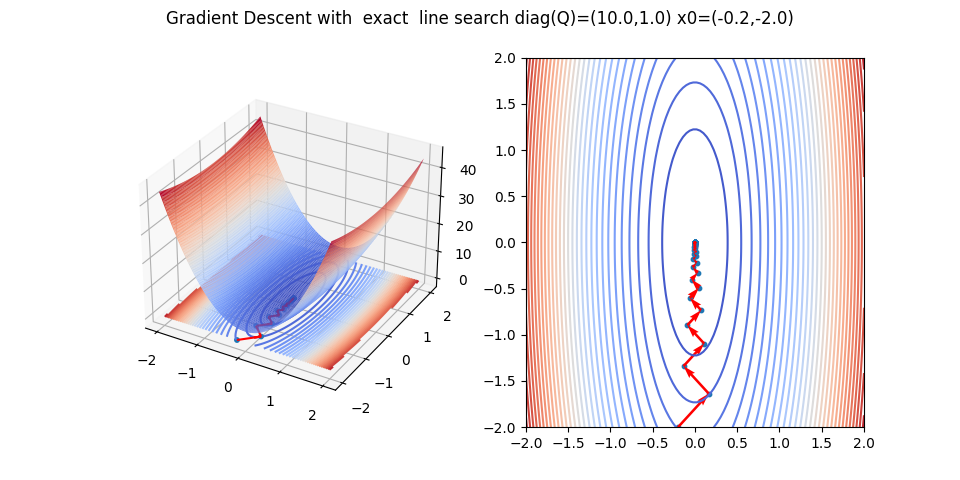
\includegraphics[scale=0.5]{grad_descent_exact_1.png}\\
We can see that we are zigzaging when going at the steepest descent direction. this is since the next direction will always be orthogonal to the current one (directional derivative result of exact line search $\nabla f^T r = 0$ ). this is also related to the convergence rate constant $1 - \frac{\lambda_{min}}{\lambda_{max}}$. In our case it is close to $1$, therefore we converge slowly. In this case we converged after $\bold{63}$ iterations.\\
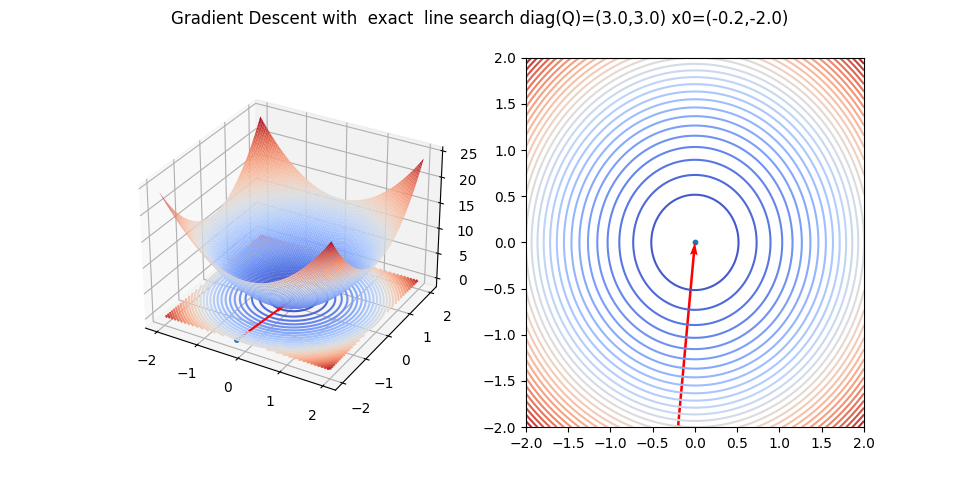
\includegraphics[scale=0.5]{grad_descent_exact_2_circle.png}
When the hessian eigen values are the same $\lambda_{min} = \lambda_{max} = 3$, we don't zigzag and with only one iteration we find the minimum. this is related to the convergence rate constant $1 - \frac{\lambda_{min}}{\lambda_{max}}$. In our case it is 0, therefore we converge after $\bold{1}$ iteration.\\
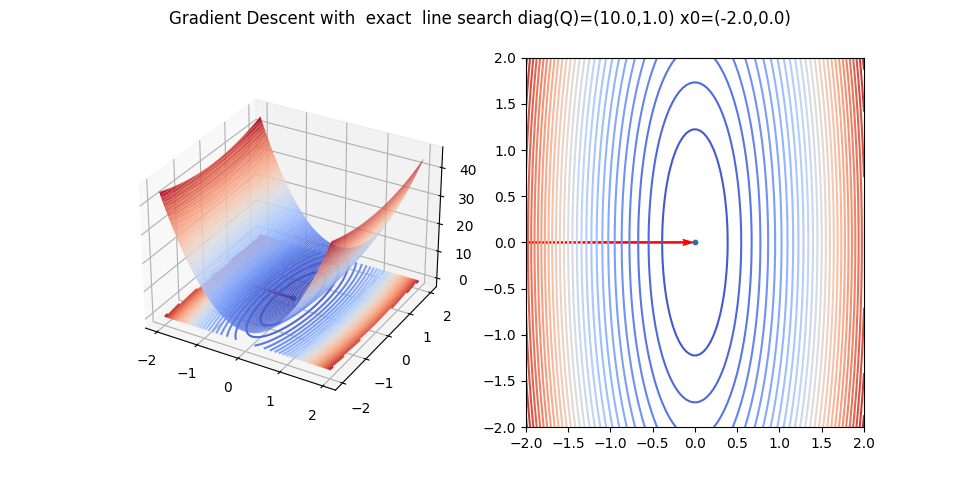
\includegraphics[scale=0.5]{grad_descent_exact_3_elipse_easy_start_point.png}
When starting at an ideal point where the directional derivative is directed right to the global minimum. In such a case we converge after $\bold{1}$ iteration.\\
\subsubsection{The results of Gradient Descent with inexact line search:}
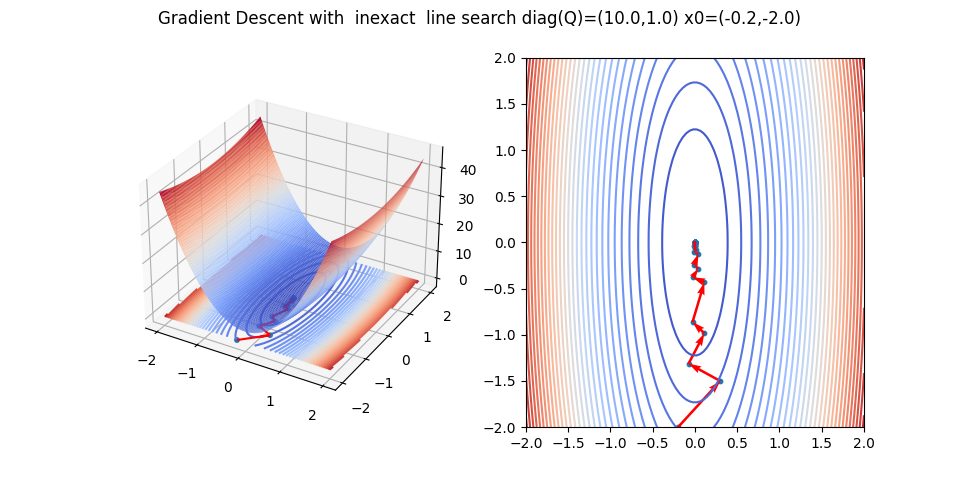
\includegraphics[scale=0.5]{grad_descent_inexact_1.png}
With inexact line search, we zigzag less than steepest descent as we don't go to the exact minimum in which we will have an orthogonal next direction, but rather find better step size according to armijo rule. In this case we converged after $\bold{45}$ iterations.\\
\newpage
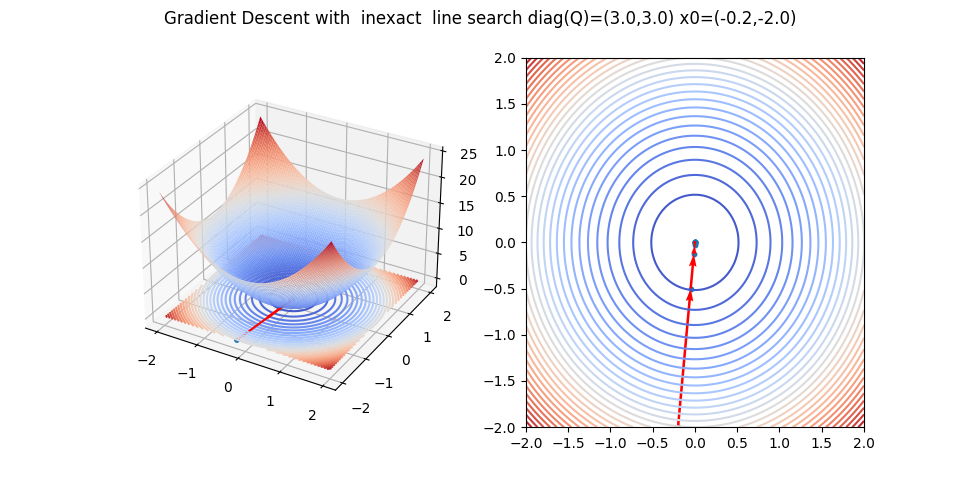
\includegraphics[scale=0.5]{grad_descent_inexact_2_circle.png}
When the hessian eigen values are the same $\lambda_{min} = \lambda_{max} = 3$, we can see worse performance of inexact line search compared to exact, as in this case inexact oscillate around the minimum point due to its use of inexact step size to reach the minimum in one step. In this case we converged after $\bold{10}$ iterations.\\
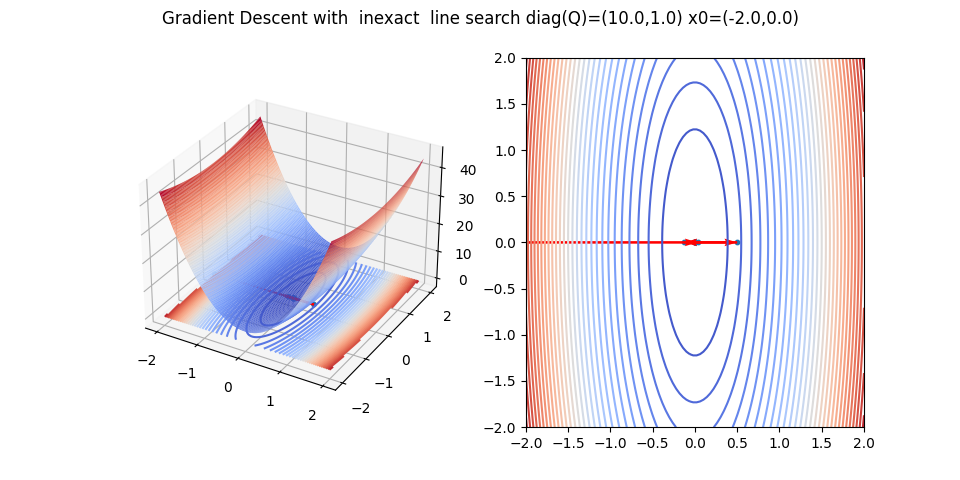
\includegraphics[scale=0.5]{grad_descent_inexact_3_elipse_easy_start_point.png}
Similar to previous case, we can see that the performance is worse compared to exact line search and we oscillate. In this case we converged after $\bold{11}$ iterations.\\

\subsubsection{The results of Newton method with exact/inexact line search:}
At all runs of newton method, we converged after a single iteration. These results are due to the fact that we try to optimize a quadratic function and in newton method the quadratic approximation calculated matches exactly the actual function. Thus, by calculating the correct direction/displacement to the minimum and following exact line search, we hit the optimum directly.\\
Also, on inexact line search we do not oscillate since we start with $\alpha_0=1$ in which we start at the exact approximation of the displacement for the quadratic function.\\
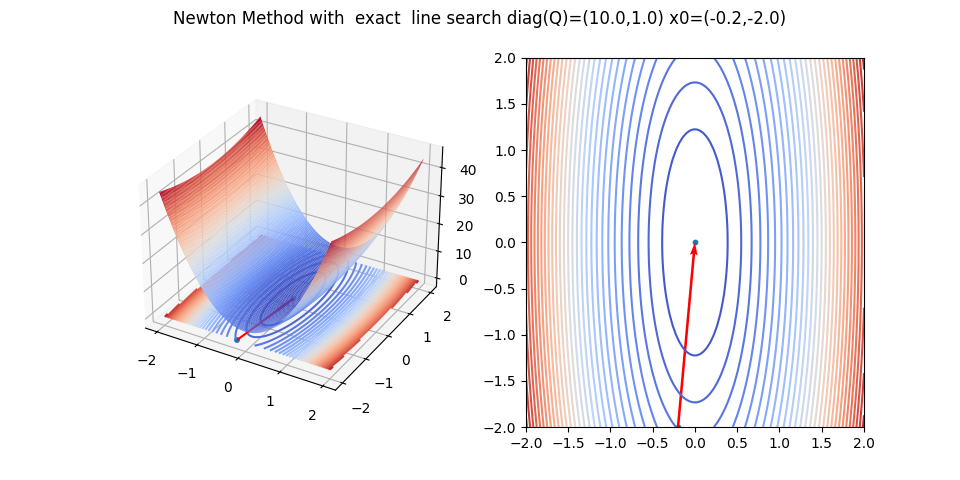
\includegraphics[scale=0.5]{nm_exact_1.png}\\
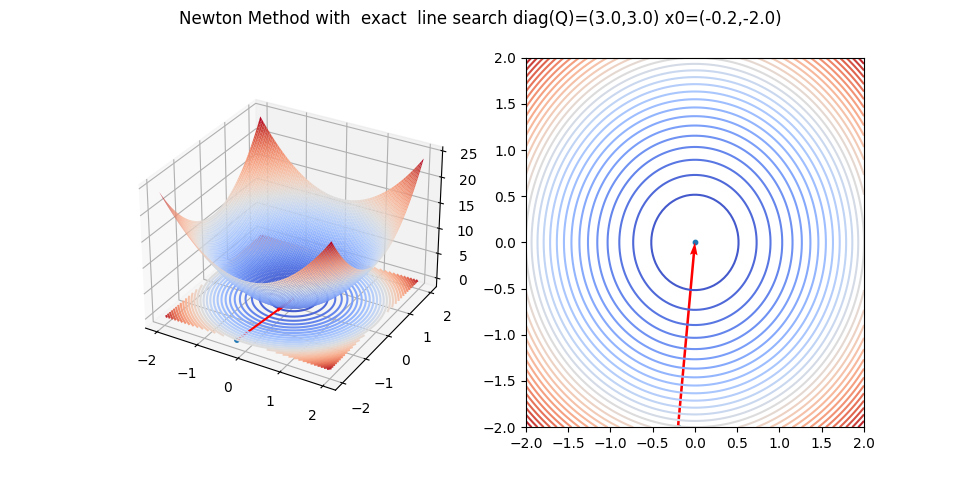
\includegraphics[scale=0.5]{nm_exact_2_circle.png}\\
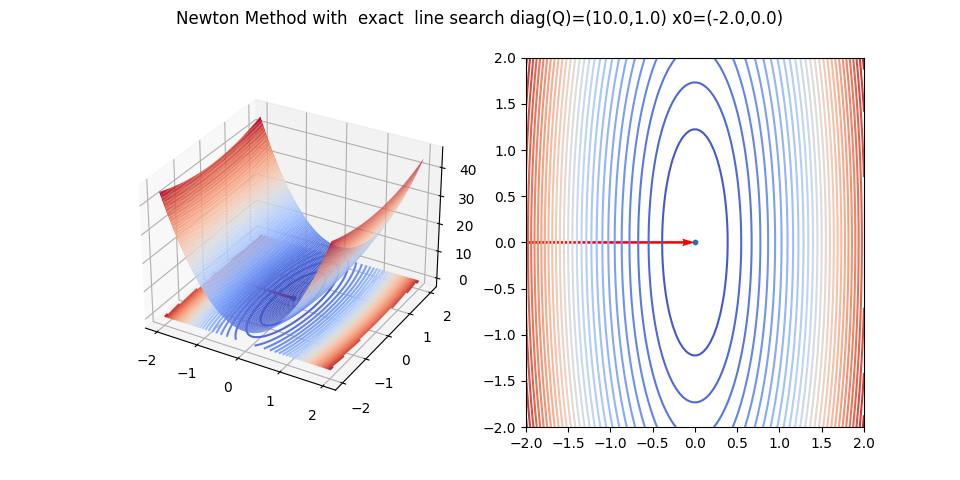
\includegraphics[scale=0.5]{nm_exact_3_elipse_easy_start_point.png}\\
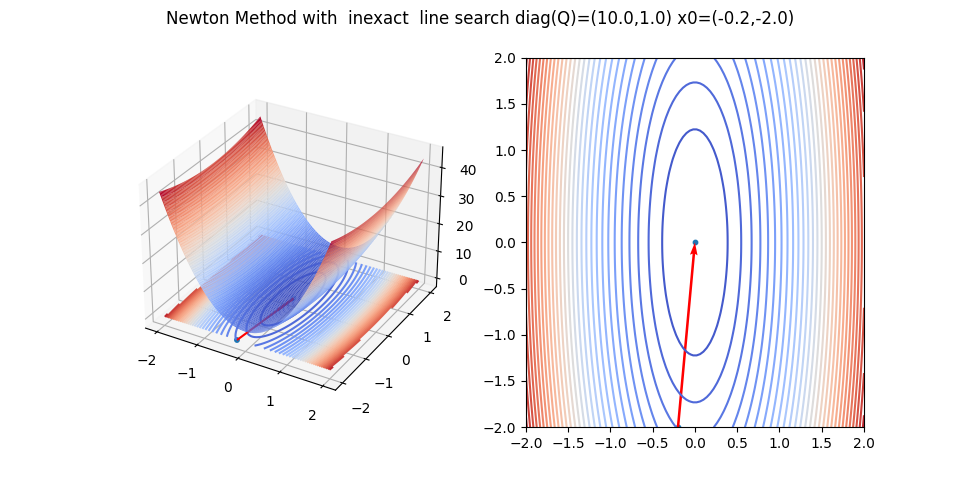
\includegraphics[scale=0.5]{nm_inexact_1.png}\\
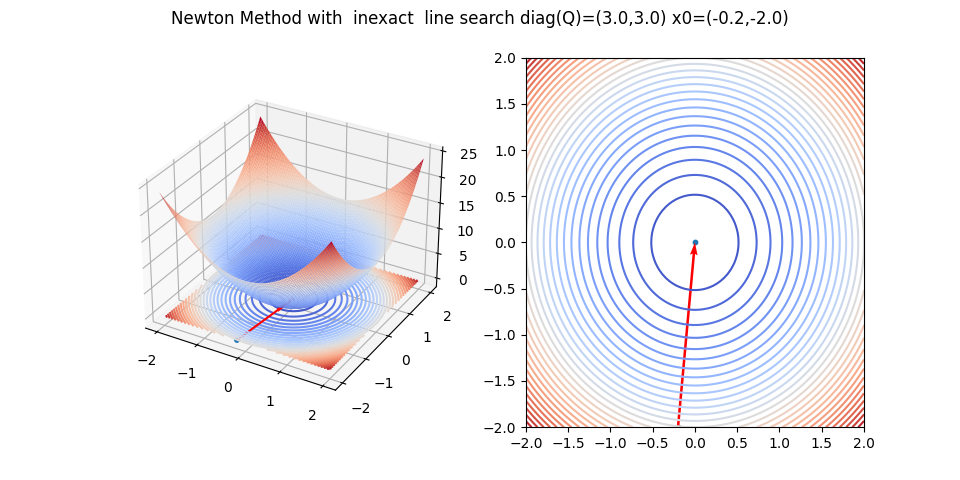
\includegraphics[scale=0.5]{nm_inexact_2_circle.png}\\
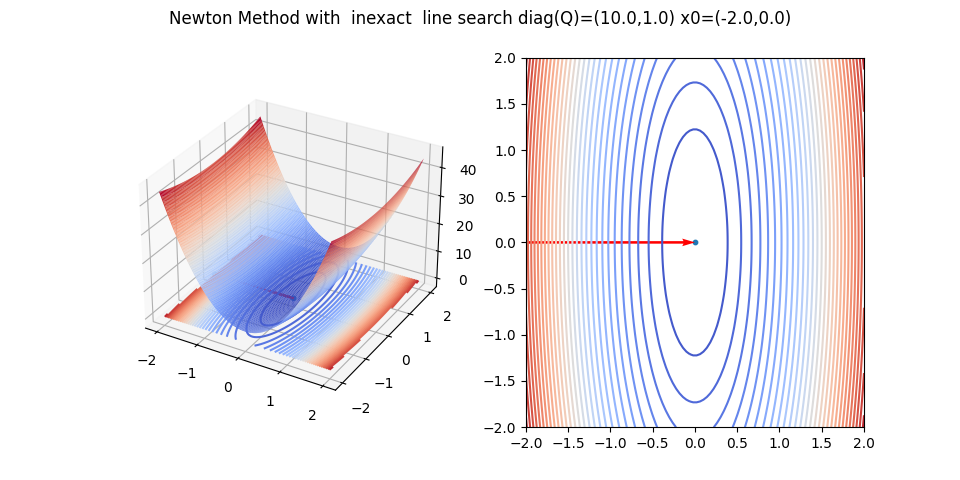
\includegraphics[scale=0.5]{nm_inexact_3_elipse_easy_start_point.png}\\
\subsection{}
\subsection{Find  the  Minimum  of  the  Rosenbrock  Function}
The Rosenbrock function gets its minimum at $x = (1,1,1...,1)$ point. we can calculate the value and see that it is 0. which is the minimum as $$Rosenbrock\_f(x) \geq 0\; \forall x \in \mathbb{R}^n$$
Therefore, the difference to optimal value is actualy the function value at each trajectory point in our search for the optimal point.\\
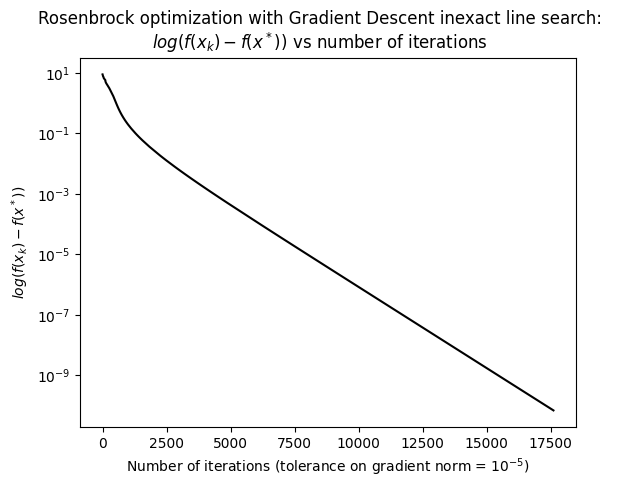
\includegraphics[scale=0.5]{r_f_gd.png}\\
We can see a linear convergence rate for the Gradient Descent algorithm. As we get a $10^-2$ decrease relative to a constant rate of iterations.
In this method we've run for 17612 iterations (the Rosenbrock function is a test bench to compare between optimization methods as it is hard to find the optimal point)\\
\newpage
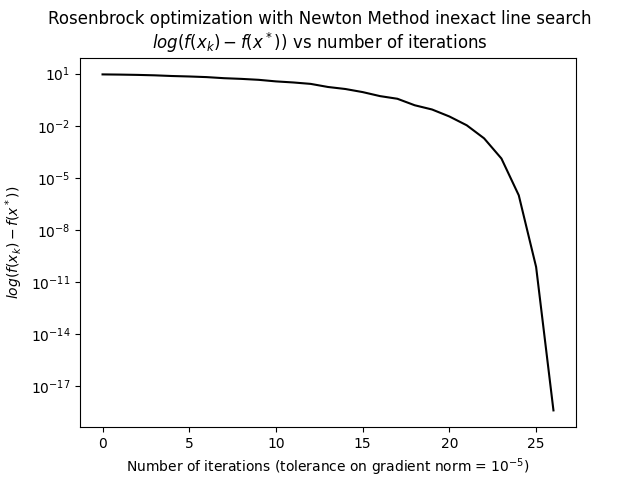
\includegraphics[scale=0.5]{r_f_nm.png}\\
We can see an asymptotic convergence rate for the Newton Method algorithm. When we reach close enough to minimum point, the rate of convergence accelerate polynomialy (or even exponentially) and we get fast decreases of $10^{-2},10^{-4},10^{-8}..$ relative to a constant rate of iterations.\\
In this method we've run for 26 iterations and converged.

\end{document}

